\chapter{\uppercase{Simulation Results}}



\begin{figure}[t!]
  \centering
  \def\svgwidth{0.7\columnwidth}
  \input{figs/cart_spring.eps_latex}
  \caption[Configuration of the cart--spring system.]{Configuration of the
    cart--spring system.}
  \label{fig:cart-spring-configuration}
\end{figure}

\section{Cart--Spring System}

The simplest example system to which energy shaping can be applied is a system
with a one-dimensional configuration space.
%
The cart--spring system shown in \figref{fig:cart-spring-configuration} is just
such a system and can be used to build intuition into the methods presented.

\subsection{Setup}

This well-known example is highly idealized and assumes rolling without slipping
and no damping.
%
As shown in \figref{fig:cart-spring-configuration}, the cart has mass $M$ and is
acted on by an idealized spring with stiffness $K$.
%
It is assumed that (by turning the wheels) a force can be applied directly along
the $x$-axis in the same way in which the spring acts.

%
Parameterizing the motion of the system by the horizontal displacement, $\q$, with
associated velocity $\dq$, leads to the configuration space $\Q = \R$ with
tangent bundle $T\Q = \R^{2}$ which has coordinates $\x = \argsqdq \in \T\Q$.
%
Disregarding physical restrictions on spring length leads to the domain of
admissibility for the system being entire, i.e., $\D = \R^{2}$.
%
The dynamics of the system obeys the differential equation
\begin{align*}
  M \ddq + K \q = \uu
\end{align*}
where $M$ is the mass of the cart, $K$ is the spring constant, and $u$ is the
control force in newtons.

This system is not intrinsically a hybrid system and, as a result, energy
shaping cannot be directly applied.
%
However, this system can be made amenable to energy shaping by embedding it
in a hybrid system.
%
Consider that the motion of the spring--cart system involves oscillation about
the origin.
%
Thus all non-trivial trajectories pass through the origin repeatedly, so a
natural choice for the switching surface (\Poincare{} section) is the set
\begin{align}
  \Guard = \left\{ \argsqdq \in T\Q : \q = 0 \mbox{ and } \dq < 0 \right\}.
  \label{eq:cart_spring_guard}
\end{align}
%
Using this switching surface with the domain of admissibility specified above
permits reformulation of the cart--spring system as a hybrid system:
%
\begin{align}
  \HCS = \left\{
  \begin{array}{l l}
    \dx\hphantom{^+} = \xf\argsqdq + \xg \, \uu, & \argsqmdqm \in \D \setminus
    \Guard,\\
    \xp = \argsqmdqm, & \argsqmdqm \in \Guard,
  \end{array}\right.
\end{align}
where
\begin{align*}
  \xf\argsqdq = \left(\begin{array}{c}
      \dq\\
      -\frac{K}{M} \q
    \end{array}\right), \qquad
    \xg = \left(\begin{array}{c}
        0\\
        \frac{1}{M}.
      \end{array}\right).
\end{align*}

For the constructed hybrid system, the discrete dynamics for the configuration
and velocity do not change.
%
Moreover, with no control input, the system is conservative and does not exhibit
asymptotic stability.
%
In order to demonstrate the application of energy shaping, a limit cycle can be
induced in the system using, for example, the same dissipation present in the
Van der Pol oscillator (see \cite[pp.~13]{Khalil2002}).
%
As described in \chapref{ch:energy-shaping}, the state of the system can be
augmented to include a storage function for energy flow due to non-conservative
forcing, i.e.,
\begin{align*}
  \x = \argsqdqW
\end{align*}
where $W$ is the energy storage function as in \eqref{eq:ncsys-nrg-cons}.
%
Applying the feedback control law
\begin{align}
  \label{eq:spring_cart_vdp_controller}
  \uu = \vv\argsqdq = \gamma(1 - \q^{2}) \, \dq + w
\end{align}
with $\gamma = .2$ leads to the hybrid control system
\begin{align}
  \label{eq:hcs_cart_spring}
  \HCSbar = \left\{
  \begin{array}{l l}
    \dx\hphantom{^+} = \xfbar\argsqdq + \xgbar \, w, & \argsqmdqm \in \D \setminus \Guard,\\
    \xp = \Delta\argsqmdqm, & \argsqmdqm \in \Guard,
  \end{array}\right.
\end{align}
where the nominal controller is subsumed under the system dynamics and energy
flow is tracked in the $W$ coordinate, viz.
\begin{align*}
  \xfbar\argsqdq = \left(\begin{array}{c}
      \dq\\
      -\frac{K}{M} \q + \frac{1}{M} \gamma(1 - \q^{2}) \, \dq\\
      \gamma(1 - \q^{2}) \, \dq^{2}
    \end{array}\right), \qquad
  \xgbar\argsdq = \left(\begin{array}{c}
      0\\
      \frac{1}{M}\\
      0
    \end{array}\right),
\end{align*}

and the reset map acts to reset the stored energy, i.e.,
\begin{align*}
  \Delta\argsqdq = (\q, \dq, 0).
\end{align*}

\begin{figure*}[htp!]
  \centering
  \includegraphics[width=0.85\textwidth]{hybrid_cart_spring_phase_portrait}
  \includegraphics[width=0.85\textwidth]{hybrid_cart_spring_coordinates}
  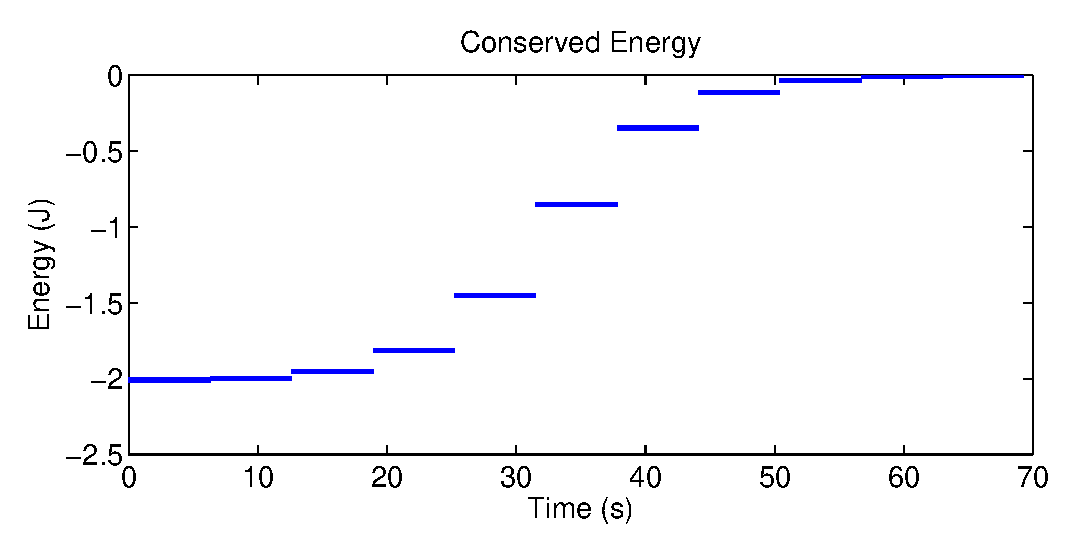
\includegraphics[width=0.85\textwidth]{hybrid_cart_spring_energy}
  \caption[Simulation of the nominal cart--spring system.]{Simulation of the
    nominal cart--spring system.
    % 
    A force from the nominal control law \eqref{eq:spring_cart_vdp_controller}
    acts on the cart.
    %
    Top: phase portrait demonstrating the existence of a limit cycle;
    %
    middle: evolution of the state coordinates;
    %
    bottom: the conserved energy jumps when the storage function is reset at the
    switching surface.}
  \label{fig:cart_spring_simulation_nominal}
\end{figure*}

\subsection{Simulation of Nominal System}
Beginning from the (post-reset) initial condition
\begin{align*}
  \argsqdqW = (0, -.1, 0),
\end{align*}
a simulation was conducted to illustrate the nominal behavior of cart--spring
system governed by \eqref{eq:hcs_cart_spring} under the Van der Pol controller
defined in \eqref{eq:spring_cart_vdp_controller} with $w = 0$;
%
that is, the closed-loop hybrid system
\begin{align}
  \label{eq:hs_cart_spring_nominal}
  \HSbar = \left\{
    \begin{array}{l l}
      \dx\hphantom{^+} = \xfbar\argsqdq, & \argsqmdqm \in \D \setminus \Guard,\\
      \xp = \Delta\argsqmdqm, & \argsqmdqm \in \Guard,
    \end{array}\right.
\end{align}
%
The simulation was constructed to terminate when the distance between successive
crossings of the \Poincare{} section \eqref{eq:cart_spring_guard} dropped below
a threshold---in this case, $10^{-3}$---which served as the convergence
criterion.
%
From \figref{fig:cart_spring_simulation_nominal}, it is apparent that the
simulation lasted just under $70$ seconds.
%
The phase portrait in \figref{fig:cart_spring_simulation_nominal} shows that the
system eventually converges to a limit cycle over relatively large number of
steps (i.e., iterations of the \Poincare{} first return map).
By counting the jumps in the plot of conserved energy in
\figref{fig:cart_spring_simulation_nominal}, one can see that convergence based
on the aforementioned criterion requires 11 ``steps'';
%
in other words, the cart passes through the origin from the positive side 11
times.


From the evolution of the coordinates shown in
\figref{fig:cart_spring_simulation_nominal}, it is apparent that the
oscillations grow until the system reaches the limit cycle.
%
The conserved energy of the limit cycle (as defined in
\eqref{eq:cart_spring_guard}) can be seen to change between iterations in \figref{fig:cart_spring_simulation_nominal}.
%
This jump is a result of the resetting of the storage function, $W$, which
occurs when the cart passes through the switching surface
\eqref{eq:cart_spring_guard}.

\begin{figure*}[htp!]
  \centering
  \includegraphics[width=0.85\textwidth]{hybrid_cart_spring_es_phase_portrait}
  \includegraphics[width=0.85\textwidth]{hybrid_cart_spring_es_coordinates}
  \includegraphics[width=0.85\textwidth]{hybrid_cart_spring_es_energy}
  \caption[Simulation of the shaped cart--spring system.]{Simulation of the
    shaped cart--spring system.
    %
    A force from the nominal control law \eqref{eq:spring_cart_vdp_controller}
    acts on the cart along with a force from energy shaping.
    % 
    Top: phase portrait demonstrating the existence of a limit cycle and rapid
    stabilization;
    %
    middle: evolution of the state coordinates;
    %
    bottom: the conserved energy stabilizes to the desired value at an
    exponential rate.}
  \label{fig:cart_spring_simulation_shaped}
\end{figure*}

\subsection{Simulation of Shaped System}
